\documentclass{article}
\usepackage[utf8]{inputenc}
\usepackage{tikz}
\usepackage{amsmath}
\usepackage{amssymb}
\tikzset{v/.style = {circle, thick, minimum size=2.0mm, inner sep=0pt, draw},
    a/.style = {        thick, minimum size=2.0mm, inner sep=0pt, draw},
    b/.style = {circle, fill,  minimum size=1.8mm, inner sep=0pt, draw},
    d/.style = {}}


\title{COMP3940 Auto Generated Example Test}
\author{https://github.com/rnash-01/3940-practice}
\date{January 2023}


\begin{document}

\maketitle
\section{Network Flow}
\subsection*{Question 1.1}Find the maximum flow and minimum cut in the graph below
\begin{center}
  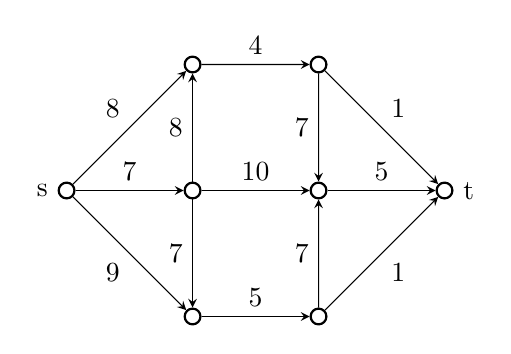
\begin{tikzpicture}[scale=0.8, >=stealth]
    \node[v, label=left :s] (s) at (0,2) {}; 
    \foreach \n/\y in {a/0, b/2, c/4} \node[v] (\n) at (2,\y) {};
    \foreach \n/\y in {d/0, e/2, f/4} \node[v] (\n) at (4,\y) {};
    \node[v, label=right:t] (t) at (6,2) {};

    \draw[->] (s) to[edge label'=9] (a);
    \draw[->] (s) to[edge label =7] (b);
    \draw[->] (s) to[edge label =8] (c);
    \draw[->] (b) to[edge label'=7] (a);
    \draw[->] (b) to[edge label =8] (c);
    \draw[->] (a) to[edge label =5] (d);
    \draw[->] (b) to[edge label =10] (e);
    \draw[->] (c) to[edge label =4] (f);
    \draw[->] (d) to[edge label =7] (e);
    \draw[->] (f) to[edge label'=7] (e);
    \draw[->] (d) to[edge label'=1] (t);
    \draw[->] (e) to[edge label =5] (t);
    \draw[->] (f) to[edge label =1] (t);\end{tikzpicture}
\end{center}
\section{Matchings}
\subsection*{Question 2.1}For the following graphs and matchings select which are matchings and which are not. For each, if they are a matching, state whether or not they have an augmenting path.

\subsubsection{1}
\begin{center}
    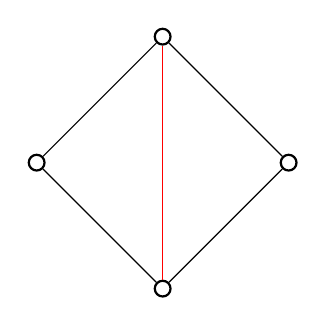
\begin{tikzpicture}[scale=0.8, >=stealth]
        \node[v] (a) at (0,2) {}; 
        \foreach \n/\y in {b/0, c/4} \node[v] (\n) at (2,\y) {};
        \node[v] (d) at (4,2) {};

        \draw  (b) -- (d);
        \draw  (a) -- (b);
        \draw  (c) -- (d);
        \draw [color=red] (b) -- (c);
        \draw  (a) -- (c);
    \end{tikzpicture}
\end{center}

\subsubsection{2}
\begin{center}
    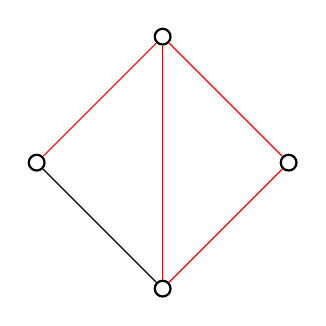
\begin{tikzpicture}[scale=0.8, >=stealth]
        \node[v] (a) at (0,2) {}; 
        \foreach \n/\y in {b/0, c/4} \node[v] (\n) at (2,\y) {};
        \node[v] (d) at (4,2) {};

        \draw [color=red] (b) -- (d);
        \draw  (a) -- (b);
        \draw [color=red] (c) -- (d);
        \draw [color=red] (b) -- (c);
        \draw [color=red] (a) -- (c);
    \end{tikzpicture}
\end{center}

\subsubsection{3}
\begin{center}
    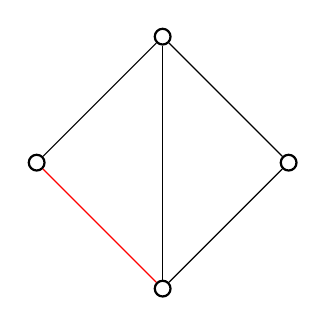
\begin{tikzpicture}[scale=0.8, >=stealth]
        \node[v] (a) at (0,2) {}; 
        \foreach \n/\y in {b/0, c/4} \node[v] (\n) at (2,\y) {};
        \node[v] (d) at (4,2) {};

        \draw  (b) -- (d);
        \draw [color=red] (a) -- (b);
        \draw  (c) -- (d);
        \draw  (b) -- (c);
        \draw  (a) -- (c);
    \end{tikzpicture}
\end{center}

\subsubsection{4}
\begin{center}
    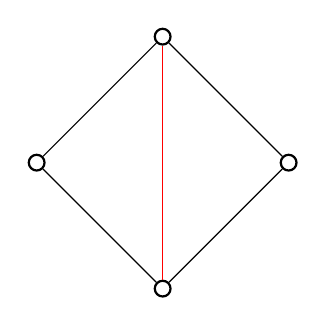
\begin{tikzpicture}[scale=0.8, >=stealth]
        \node[v] (a) at (0,2) {}; 
        \foreach \n/\y in {b/0, c/4} \node[v] (\n) at (2,\y) {};
        \node[v] (d) at (4,2) {};

        \draw  (b) -- (d);
        \draw  (a) -- (b);
        \draw  (c) -- (d);
        \draw [color=red] (b) -- (c);
        \draw  (a) -- (c);
    \end{tikzpicture}
\end{center}

\section{Complexity Theory}
\subsection*{Question 3.1}Consider 3 problems: $\Pi \in \mathbb{P}$, $\Psi \in \mathbb{NP}$, and $\Phi \in \text{co-}\mathbb{NP}$. Assuming that $\mathbb P \ne \mathbb{NP}$, which of the following statements are true?
\subsubsection{}
$\Pi\cap\Phi\in\mathbb{P}$
\subsubsection{}
$\Phi\cup\Pi\in\mathbb{NP}$
\subsubsection{}
$\Phi\cap\Pi\in\mathbb{P}$
\end{document}